\documentclass[xcolor=dvipsnames]{beamer}

% --- Custom "Smash Ultimate" Theme ---
\usetheme{Metropolis} % Requires the metropolis theme, or fallback to 'Berlin'
\usecolortheme{rose}

% Custom Colors
\definecolor{SmashRed}{RGB}{193, 18, 31}
\definecolor{SmashGold}{RGB}{253, 184, 19}
\definecolor{SmashDark}{RGB}{20, 20, 20}

\setbeamercolor{palette primary}{bg=SmashDark, fg=white}
\setbeamercolor{palette secondary}{bg=SmashRed, fg=white}
\setbeamercolor{structure}{fg=SmashRed}
\setbeamercolor{titlelike}{parent=palette primary, fg=SmashRed}

% --- Packages ---
\usepackage[utf8]{inputenc}
\usepackage[spanish, mexico]{babel}
\usepackage{graphicx}
\usepackage{booktabs}

% --- Title ---
\title{Predicci\'on de victorias en partidas 1v1 de Super Smash Bros Ultimate}
\subtitle{Proyecto final de Aprendizaje Autom\'atico}
\author{
	Miguel Ciavato C.I. 30541929 \\
	Jhonatan Homsany C.I. 30.182.893
}
\date{Marzo, 2026}

\begin{document}
	
	\frame{\titlepage}
	
	\section{Contexto}
	\begin{frame}{Contexto}
		\begin{itemize}
			\item Super Smash Bros Ultimate (SSBU) es un videojuego de lucha desarrollado por Nintendo, es el crossover más grande de la industria.
			\item Actualmente, el juego cuenta con 87 personajes jugables contando los DLC's.
			\item El videojuego se adapta a todo tipo de jugadores.
			\item Aunque cuenta con $103$ escenarios para los combatos, los torneos competitivos suelen reducir este conjunto.
		\end{itemize}
	\end{frame}
	
	\begin{frame}{Contexto}
		\begin{itemize}
			\item Todos los jugadores comienzan en "la llave de los ganadores".
			\item En esta llave, se hacen enfrentamientos con sets se 3,5 o 7 partidas.
			\item Si un jugador pierde, pasa a la llave de perdedores. Si vuelve a perder, estando en esta llave, es descalificado.
			\item En la final, el mejor jugador de la llave de ganadores, juega contra el mejor de la llave de perdedores.
		\end{itemize}
	\end{frame}
	
	\begin{frame}{Contexto}
		\begin{figure}[h!]
			\centering
			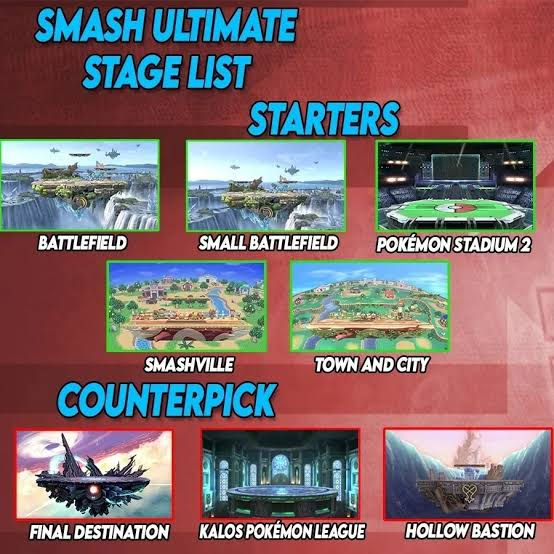
\includegraphics[width=0.5\linewidth]{figs/escenarios.png}
			\caption{Escenarios usados comunmente en competencias}
			\label{fig:escenarios}
		\end{figure}
	\end{frame}
	
	
	\begin{frame}{Contexto}
		\begin{itemize}
			\item En la primera partida, están disponibles únicamente los escenarios starters.
			\item Acá, un jugador elimina de la lista un escenario y luego el otro elimina dos. En este punto, estarán disponibles tres escenarios que pueden ser seleccionados por el jugador que realizó el primer bloqueo.
			\item Tras la primera partida, están disponibles los escenarios en ``counterpick'' y se repite el procedimiento de eliminación y selección de la primera partida.
		\end{itemize}
	\end{frame}
	
	% --- Muestreo ---
	\section{Muestreo}
	\begin{frame}{Muestreo}
		\begin{block}{Recolecci\'on de Datos}
			Para obtener los datos, se us\'o la web de \textbf{start.gg} (una plataforma de esports), que tiene una API accesible desde GraphQL para consultar datos sobre los eventos que se realizan ahí.
		\end{block}
		
		\begin{itemize}
			\item Se filtraron los torneos que tuvieran 100 participantes o más, para evitar torneos de bots o de prueba.
			\item Se usaron datos exclusivamente a partir de \textbf{2022}, ya que en ese año hubo un parche, por lo que la data previa no es válida.
			\item Se tomaron eventos de 2000 torneos aleatoriamente, para evitar sesgos de jugadores específicos o regiones.
			\item Como resultado, se obtuvieron 100.000 registros de partidas individuales (1 vs 1).
		\end{itemize}
	\end{frame}
	
	\begin{frame}{Muestreo}
		Cada una de las entradas del dataset, tiene estas características:
		\begin{itemize}
			\item El orden del juego (numero de la partida).
			\item El nombre del escenario en el que se jugó la partida.
			\item El nombre de cada jugador.
			\item El nombre del personaje que usó cada jugador.
			\item Un campo para indicar si el jugador 1 ganó.
		\end{itemize}
	\end{frame}
	
	% --- SECTION E: EXPLORE ---
	\section{Exploración}
	\begin{frame}{Exploración (Power Index)}
		\begin{itemize}
			\item Antes de pasar al preprocesamiento de los datos, se visualizaron estadísticas del dataset para entender mejor el contexto de los datos.
			\item Lo primero que se hizo fue ver qué personajes eran los "mejores", esta métrica es difícil puesto que una proporción de $\frac{victorias}{partidas}$ usada como métrica, penaliza a aquellos personajes que se usan más y eleva mucho a personajes muy poco usados con los que especialistas siempre terminan ganando.
		\end{itemize}
	\end{frame}
	
	\begin{frame}{Exploración (Power Index)}
		\begin{itemize}
			\item Obtener estas métricas más fiable es muy valioso para el modelo, por lo que, lo primero que se hizo fue añadir una métrica de tasa de victorias por jugador:
			
			$$\text{win\_rate} = \frac{\text{victorias reales} + (m \times C)}{\text{partidas jugadas} + m}$$
			
			\item Con $m$ siendo el número mínimo de victorias, y $C$ el promedio de victorias de todos los jugadores.
		\end{itemize}
	\end{frame}
	
	\begin{frame}{Exploración (Power Index)}
		\begin{itemize}
			\item Ahora, para determinar qué personajes son los mejores, se usaron \textbf{puntos}, un personaje gana puntos contra otro dependiendo del win\_rate de cada jugador.
			\item Por ejemplo, si un jugador con un win\_rate de $0.2$ que usa a Mario, le gana a uno con un win\_rate de $0.8$ que usa a Link, Mario obtendrá $0.8$ puntos.
			\item Este total de puntos, se divide entre el total de partidas de ese personaje, para obtener la métrica del \textbf{Power Index}
			
			$$\frac{\text{Suma de puntos}}{\text{Total de partidas}}\times \log_{10}(\text{Partidas} + 1)$$
			
			\item Esta es una de las métricas que utilizan en rankings como LumiRank y en comunidades de Reddit del juego, y está inspirada en métricas como el ELO en ajedrez. 
		\end{itemize}
	\end{frame}
	
	\begin{frame}{Exploración (Gráficas)}
		\begin{figure}[h!]
			\centering
			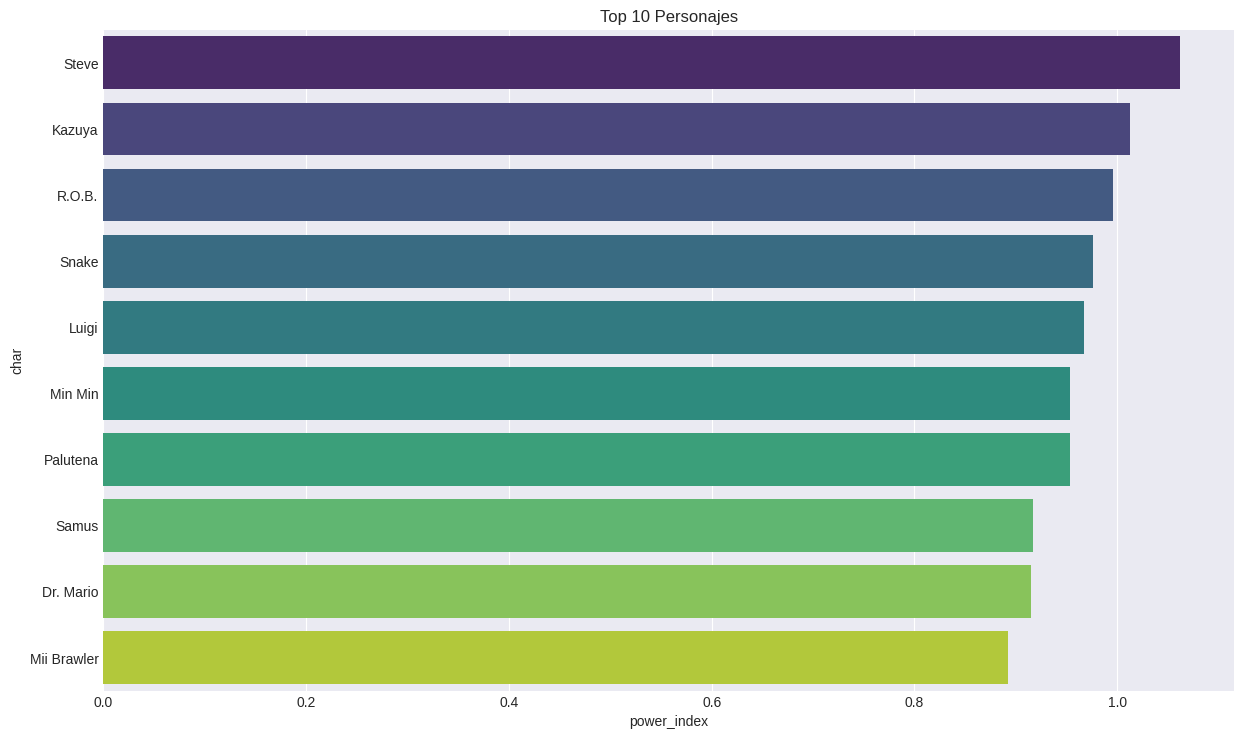
\includegraphics[width=1\linewidth]{figs/top_personajes.png}
			\caption{Top personajes según el power index}
			\label{fig:escenarios}
		\end{figure}
	\end{frame}
	
	\begin{frame}{Exploración (Gráficas)}
		\begin{figure}[h!]
			\centering
			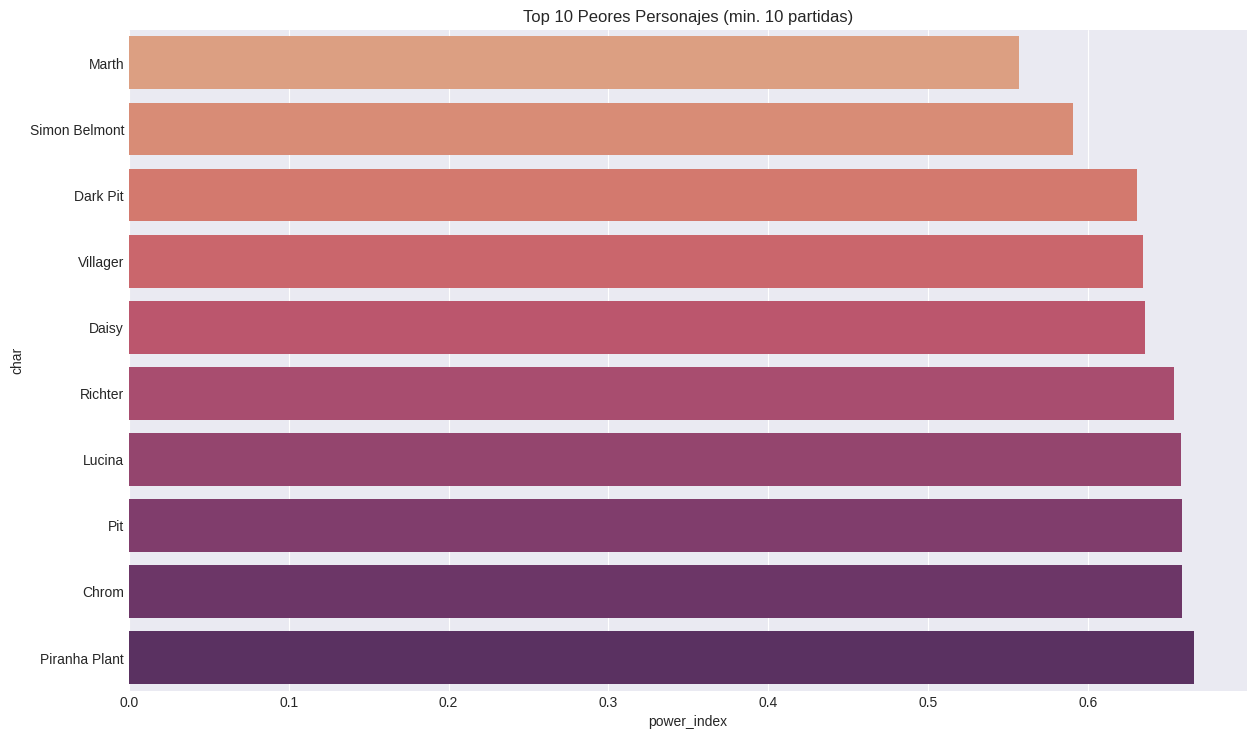
\includegraphics[width=1\linewidth]{figs/peores_personajes.png}
			\caption{Peores personajes según el power index}
			\label{fig:escenarios}
		\end{figure}
	\end{frame}
	
	\begin{frame}{Exploración (Gráficas)}
		\begin{figure}[h!]
			\centering
			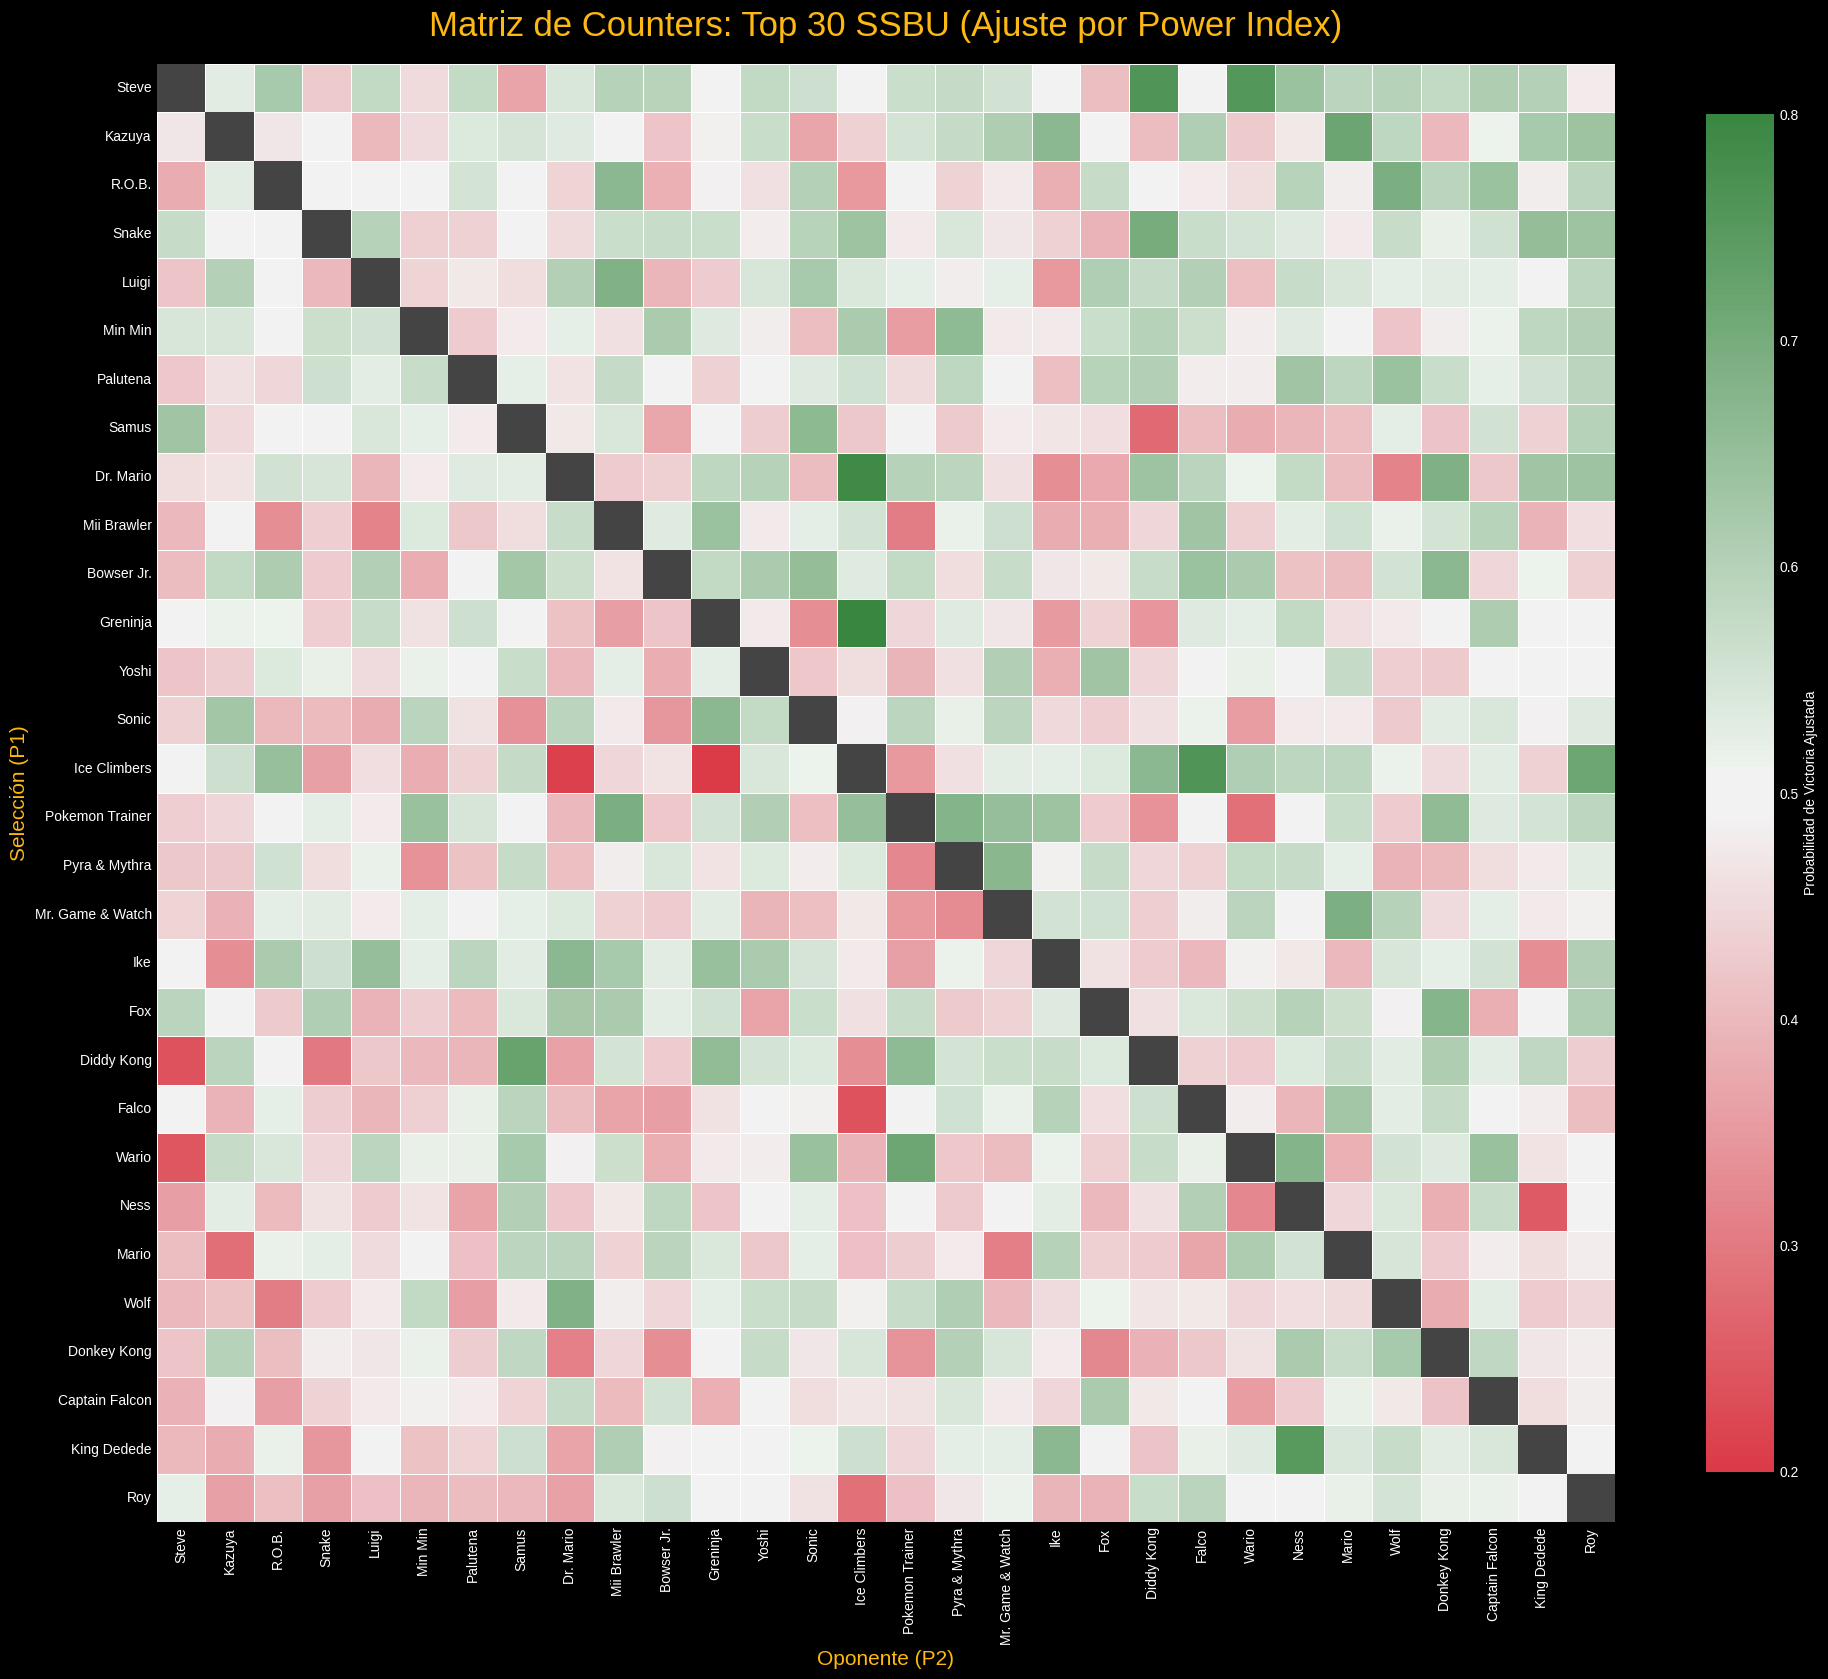
\includegraphics[width=0.7\linewidth]{figs/matriz_counter.png}
			\caption{Matriz de Match Up entre personajes}
			\label{fig:escenarios}
		\end{figure}
	\end{frame}
	
	\begin{frame}{Exploración (Gráficas)}
		\begin{figure}[h!]
			\centering
			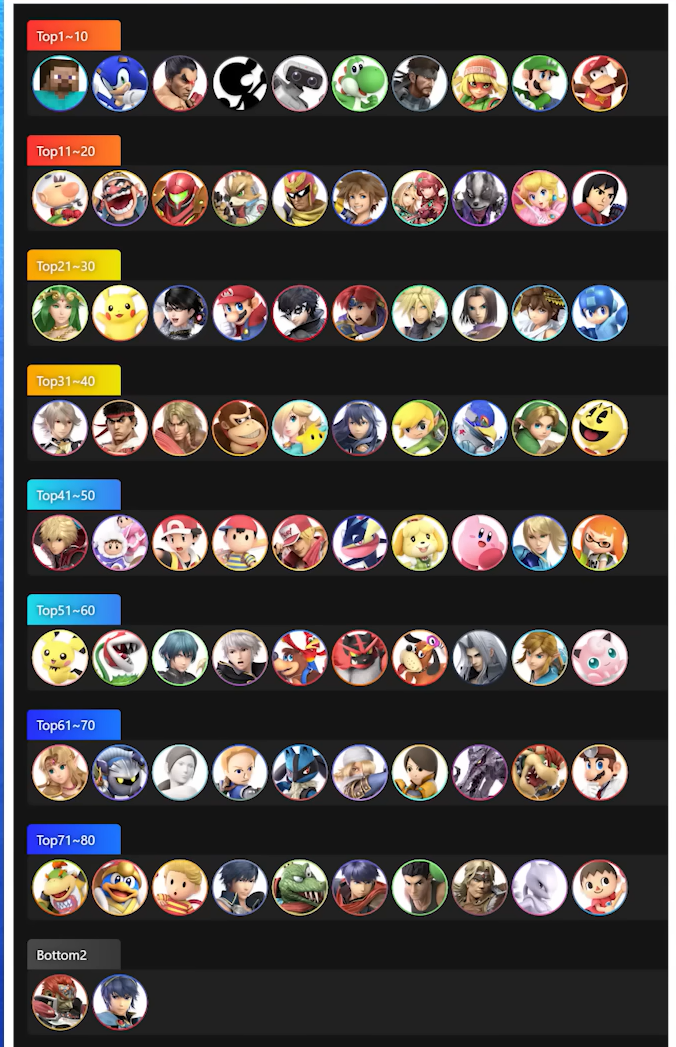
\includegraphics[width=0.4\linewidth]{figs/top_oficial.png}
			\caption{Top oficial}
			\label{fig:escenarios}
		\end{figure}
	\end{frame}
	
	\begin{frame}{Exploración (Conclusiones)}
		Todo esto se hizo como una antesala al modelo, para corroborar que:
		\begin{itemize}
			\item Existen personajes que son mejores contra otros, independientemente de la habilidad del jugador (hay un desbalance claro).
			\item El uso del win\_rate y power index tiene un potencial predictivo, ya que las estadísticas que se consiguieron son similares a las publicadas en rankings como LumiRank.
			\item Esto nos lleva a la hipótesis de que usar estás métricas, en conjunto con el escenario y número de partida pueden permitirle a un modelo hacer buenas predicciones.
		\end{itemize}
	\end{frame}
	
	% --- SECTION M: MODIFY ---
	\section{Modificación (Preprocesamiento)}
	\begin{frame}{Modificación}
		\begin{itemize}
			\item Para preprocesar los datos, inicialmente se hizo un label encoding para no usar texto en el entrenamiento.
			\item Se incluyó el \textbf{Power Index} de los personajes que usó cada jugador y el \textbf{Win-Rate} de cada jugador.
			\item Se descartaron las partidas con escenarios desconocidos.
			\item Se usó el StandardScaler para estandarizar las características, removiendo la media y escalando hasta llegar a varianza $1$.
			\item Se uso el $70\%$ de datos para el entrenamiento y el $30\%$ para prueba.
		\end{itemize}
	\end{frame}
	
	% --- SECTION M: MODEL ---
	\section{Modelado}
	\begin{frame}{Modelado (Algoritmo escogido)}
		\begin{itemize}
			\item Dadas las características de este dataset, se optó por usar un modelo de regresión logística, ideal para predecir la clase (victoria p1, derrota p1) de una partida en particular.
			\item Es importante resaltar que las predicciones del modelo se basan exclusivamente en las condiciones iniciales de la partida, por lo que no se toman en cuenta otras condiciones que puedan afectar la victoria mientras la partida está en curso.
		\end{itemize}
	\end{frame}
	
	\begin{frame}{Modelado (Regularización)}
		\begin{itemize}
			\item Lo primero que se hizo fue definir un espacio logaritmico np.logspace(-4, 2, 25), para encontrar el mejor hiperparámetro de regularización $C$ para el modelo de regresión logística en ese espacio.
			\item Se hizo uso de validación cruzada con 5 folds, balanceando las clases y usando la penalización L1.
		\end{itemize}
	\end{frame}
	
	\begin{frame}{Modelado (Regularización)}
		\begin{figure}[h!]
			\centering
			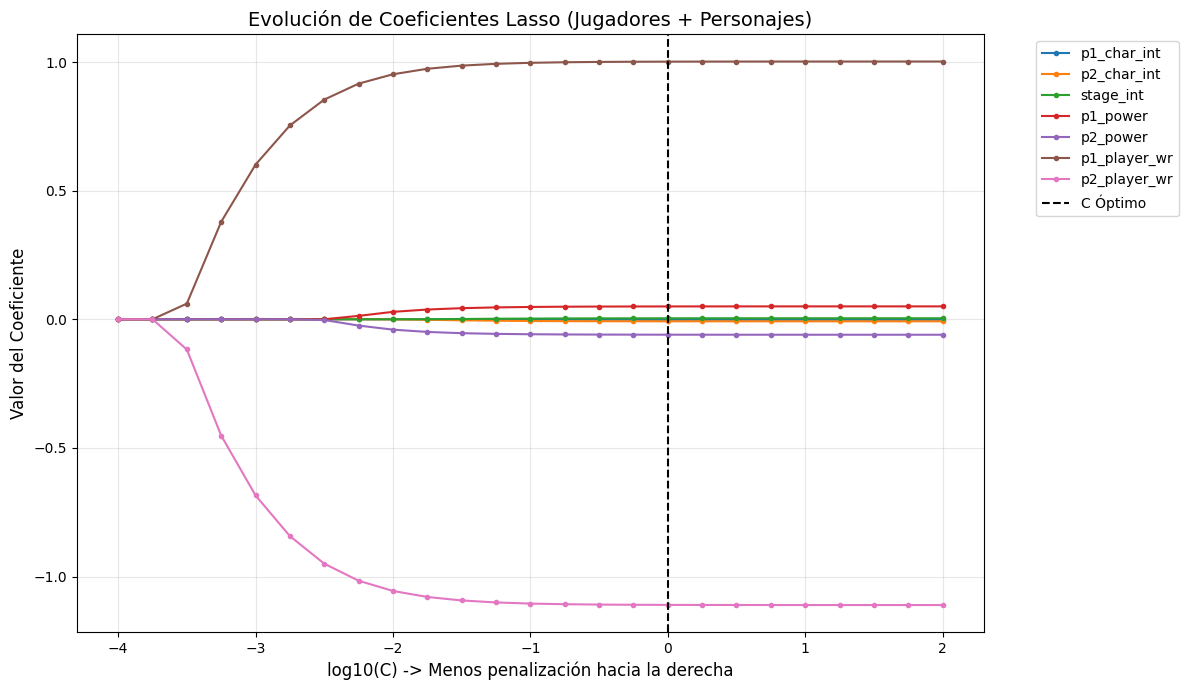
\includegraphics[width=1\linewidth]{figs/coeficientes_lasso.png}
			\caption{Evolución de coeficientes en el camino de regularización}
			\label{fig:escenarios}
		\end{figure}
	\end{frame}
	
	\begin{frame}{Modelado (Regularización)}
		\begin{itemize}
			\item El impacto de las variables tras aplicar Lasso nos indica que la mejor manera que tenemos para predecir al ganador de una partida es en base a su \textbf{consistencia} (su Win-rate), seguida de la viabilidad técnica del personaje. Seguido de esto, tenemos el impacto del escenario que si bien afecta al personaje, los jugadores más habilidosos son capaces de adaptarse a este tipo de situaciones para lograr la victoria.
		\end{itemize}
	\end{frame}
	
	\begin{frame}{Modelado (Árboles de decisión)}
		\begin{itemize}
			\item Aparte de regresión Logística, probamos otros modelos, para comparar el rendimiento
			\item Con árboles de decisión, se usó un límite de 3 niveles, con pesos de clases balanceados, utilizando el win\_rate de los jugadores como criterio para dividir los datos en cada nodo del árbol, sabiendo que estas son las variables más relevantes para la victoria.
		\end{itemize}
	\end{frame}
	
	\begin{frame}{Modelado (Árboles de decisión)}
		\begin{figure}[h!]
			\centering
			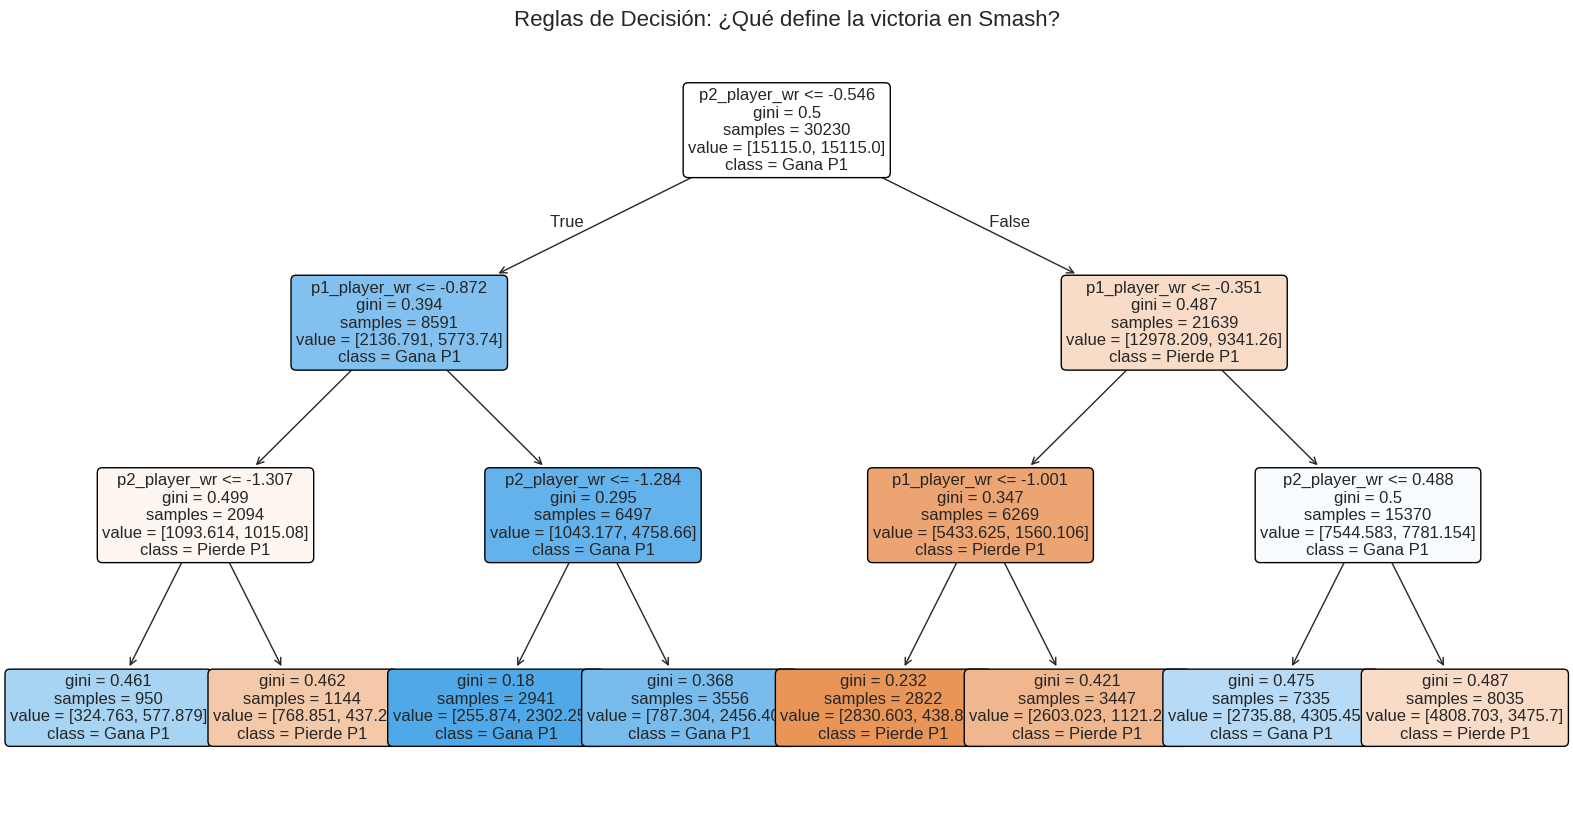
\includegraphics[width=1\linewidth]{figs/arbol.png}
			\caption{Árbol de decisión resultante}
			\label{fig:escenarios}
		\end{figure}
	\end{frame}
	
	% --- SECTION A: ASSESS ---
	\section{Evaluación}
	\begin{frame}{Evaluación}
		También se usaron Máquinas de soporte vectorial, con un peso de clases balanceado, obteniendo estos resultados:
		
		\begin{table}[]
			\centering
			\small
			\begin{tabular}{@{}lccc@{}}
				\toprule
				\textbf{Modelo} & \textbf{Tipo} & \textbf{F1-Score} & \textbf{Precisión Bal.} \\ \midrule
				\textbf{Regresión Logística} & \textbf{Supervisado} & \textbf{0.7376} & \textbf{70.95\%} \\
				Árbol de Decisión & Supervisado & 0.7012 & 68.47\% \\
				SVM & Supervisado & 0.6830 & 57.22\%
				\\ \bottomrule
			\end{tabular}
			\caption{Métricas finales de desempeño.}
		\end{table}
	\end{frame}
	
	\begin{frame}{Evaluación}
		\begin{figure}[h!]
			\centering
			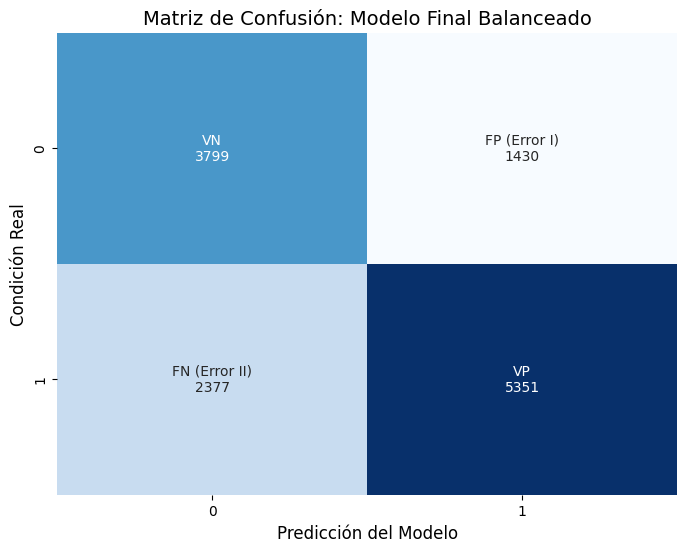
\includegraphics[width=1\linewidth]{figs/matriz_confusion.png}
			\caption{Matriz de confusión de Regresión Logística}
			\label{fig:escenarios}
		\end{figure}
	\end{frame}
	
	\begin{frame}{Conclusiones}
	\begin{itemize}
		\item La \textbf{Regresión Logística} demostró ser el modelo más robusto ($70.95\%$ de precisión y $0.73$ en Score F1), sugiriendo que la ventaja en SSBU puede modelarse de forma lineal mediante los diferentes atributos.
		\item El $30\%$ de error restante se atribuye a variables no contenidas en el dataset, como la psicología del jugador, la fatiga y la adaptación en tiempo real.
		\item Este modelo confirma que es posible predecir el éxito competitivo basándose en la ingeniería del personaje.
	\end{itemize}
	\end{frame}
	
	\section{Página web de prueba}
	
	\begin{frame}[standout]
	¡Gracias por su atención! \\
	\vspace{1em}
	\footnotesize{¿Alguna pregunta?}
	\end{frame}
	
\end{document}